%!TEX program = xelatex
\documentclass{article}
\usepackage[UTF8]{ctex}
\usepackage{authblk}
\usepackage{listings}
\usepackage{subfigure}
\usepackage{amsmath, amsfonts, amsthm, amssymb, graphicx, xcolor, hyperref, mathrsfs}
\lstset{
    basicstyle          =   \sffamily,          % 基本代码风格
    keywordstyle        =   \bfseries,          % 关键字风格
    commentstyle        =   \rmfamily\itshape,  % 注释的风格,斜体
    stringstyle         =   \ttfamily,  % 字符串风格
    flexiblecolumns,                % 别问为什么,加上这个
    numbers             =   left,   % 行号的位置在左边
    showspaces          =   false,  % 是否显示空格,显示了有点乱,所以不现实了
    numberstyle         =   \zihao{-5}\ttfamily,    % 行号的样式,小五号,tt等宽字体
    showstringspaces    =   false,
    captionpos          =   t,      % 这段代码的名字所呈现的位置,t指的是top上面
    frame               =   lrtb,   % 显示边框
}

\title{计算物理作业5} %文章标题
\author[a]{王一杰} %作者的名称
\affil[a]{中国科学技术大学}
\date{\today}%日期
\usepackage [a4paper, left=25mm,right=25mm,top=15mm,bottom=20mm]{geometry} %设置页面的环境,a4纸张大小,左右上下边距信息

\begin{document}
\maketitle
%添加这一句才能够显示标题等信息
%\tableofcontents

\section{Homework 5}
\subsection{Problem 1}

演化程序如下,很容易写出:
\begin{lstlisting}[language=MATLAB]
L=20;									%空间计算范围
T=40;									%时间计算范围
dx=0.1;									%计算空间步长
dt=0.001;								%计算时间步长
t=0:dt:T;								%时间列
x=0:dx:L;								%空间列
u=zeros(T/dt+1,L/dx+1);
u(1,1:round((L/dx+1)/2))=x(1,1:round((L/dx+1)/2));			%参数初始化
u(1,round((L/dx+1)/2):round(L/dx+1))=L-x(1,round((L/dx+1)/2):round(L/dx+1));
for i=1:1:round(T/dt)							%时间计算循环
    for j=1:1:round(L/dx+1)						%空间计算循环
        if j==1
            u(i+1,j)=0;							%边界条件
        elseif j==(L/dx+1)
            u(i+1,j)=0;							%边界条件
        else
            ut=(u(i,j+1)+u(i,j-1)-2*u(i,j))/(dx*dx);			%差分计算
            u(i+1,j)=dt*ut+u(i,j);					%一阶显式演化
        end
    end
end
\end{lstlisting}

演化结果如图1(a)所示,计算结果期望相符,图1(b)展示了$T=40$时的温度分布。需要注意的是稳定性条件要求$\frac{dt}{dx^2}<\frac{1}{2}$,而本题的取值显然满足。





\begin{figure}[tbp]
 \subfigure[时间演化过程]{\includegraphics[width=8cm]{hw5.eps}}
 \subfigure[T=40的演化结果]{\includegraphics[width=8cm]{hw52.eps}}
 \caption{Problem1的程序计算结果}
 \end{figure}

\end{document}	